\section{Neuronale Netzwerke}
%\subsection{Überblick über Neural Networks}
In den letzten Jahren hat die Technik der Neuronalen Netzwerke (Neural Networks) erneut stark an Popularität gewonnen. Dies liegt zum einen an der gestiegenen verfügbaren Rechenleistung und zum anderen an der Entwicklung hierfür notwendiger Algorithmen.\\
Es ist möglich diese Netze in zwei große Gruppen aufzuteilen: die der \textit{Feed Forward Neural Networks} und die der \textit{Recurrent Neural Networks}, welche im Folgenden als \textsc{FFNN} respektive \textsc{RNN} bezeichnet werden.\\

Ein \textsc{FFNN} besteht aus mehreren Ebenen, welche jeweils aus verschiedenen nicht-linearen Einheiten zusammengesetzt sind. Die erste dieser Ebenen wird zur Eingabe und die letzte zur Ausgabe eines Signals genutzt. Eine schematische Darstellung ist im linken Teil der Abbildung \ref{fig:ffnn_rnn_structure} zu finden. Die Einheiten zweier benachbarter Ebenen sind mit individuellen Gewichten vollständig in Richtung der Ausgabe verbunden. Dies bedeutet, dass jede Einheit $x^n_i$ ihr Signal an alle Einheiten der folgenden Ebene $x^{n+1}_j$ mit einem individuellen Gewicht $w^n_{i \rightarrow j}$ weitergibt. Zwischen den Einheiten innerhalb einer Ebene bestehen keinerlei Verbindungen.\\
Damit ein solches Netzwerk Vorhersagen treffen kann, müssen die Gewichte in einem Trainingsvorgang angepasst werden. Dies wird durch den \textit{Backpropagation}-Algorithmus erreicht. Dabei wird eine Kostenfunktion $L$ minimiert. Dies geschieht, indem die Gewichte des Netzwerkes immer in die entgegengesetze Richtung des Gradienten $\nabla_w L$ angepasst werden. Dadurch wird versucht ein Minimum der zu $L$ gehörigen Kostenlandschaft zu erreichen \cite[S. 225-290]{bishop}. Solche \textsc{FFNN} eignen sich besonders gut zur Lösung von Klassifizierungsproblemen.\\

\begin{figure}[H]
    \centering
    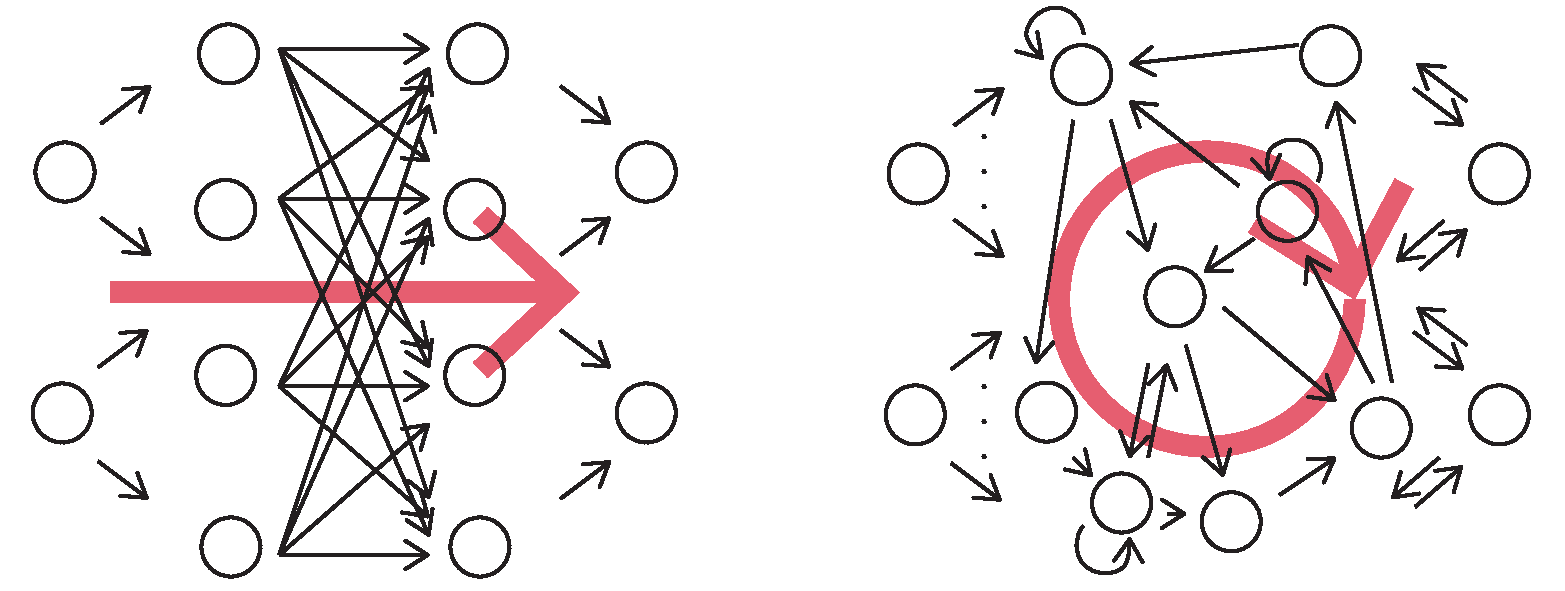
\includegraphics[width = 0.9 \textwidth]{figures/illustrations/ffnn_rnn_structure.pdf}
    \caption{Schematische Darstellung eines \textsc{FFNN} mit vier Ebenen (links) und eines \textsc{RNN} (rechts) mit ihren jeweiligen Verbindungen und der Eingangs- und Ausgangsebene. Der Informationsfluss ist in rot eingetragen (nach \citep{jeagerTut2002}).}
    \label{fig:ffnn_rnn_structure}
\end{figure}

Ein \textsc{RNN} hat einen ähnlichen Aufbau, doch hier können alle Einheiten an alle anderen Einheiten Signale weitergeben und auch von diesen erhalten. Die schematische Struktur ist im rechten Teil der Abbildung \ref{fig:ffnn_rnn_structure} dargestellt. Hierdurch erhält das Netzwerk eine Art Gedächtnisfunktion, wodurch temporale Strukturen verarbeitet und berücksichtigt werden können. Dies kann die Vorhersage in bestimmten Anwendungsbeispielen wie zum Beispiel der Text- und Sprachanalyse verbessern.\\
Ein Nachteil ist, dass zum Trainieren, aufgrund der rekurrenten Struktur, nicht mehr der einfachere \textit{Backpropagation}-Algorithmus genutzt werden kann, sondern eine für \textsc{RNN}s abgewandelte Form genutzt werden muss. Für den prominentesten Algorithmus werden die verschiedenen Zustände, die das \textsc{RNN} im Laufe der Signal-Propagation annimmt, nacheinander betrachtet und auf diese zeitliche Entwicklung anschließend der \textit{Backpropagation}-Algorithmus angewendet. Diese Methode ist unter dem Namen \textit{Backpropagation through Time} (BTT) bekannt. Sie ist zum einen rechenaufwendiger und zum anderen auch instabiler, da das Verschwinden und auch das Explodieren des Gradienten der Kostenfunktion deutlich wahrscheinlicher als bei der gewöhnlichen \textit{Backpropagation} ist \citep{pascanu, jeagerTut2002}. Da bei diesem Ansatz die Gewichte ebenfalls anhand des Gradienten der Kostenfunktion angepasst werden, wird der Algorithmus instabil, falls die Gradienten explodieren, oder ineffizient, wenn sie verschwinden.
